\documentclass[11pt,a4paper]{article}

\usepackage[T1]{fontenc}
\usepackage{lmodern}
\usepackage{microtype}
\usepackage{amsmath,amssymb,amsthm,mathtools}
\usepackage{geometry}
\usepackage{booktabs}
\usepackage{enumitem}
\usepackage{xcolor}
\usepackage{hyperref}
\usepackage{tikz}

\geometry{margin=30mm}
\hypersetup{colorlinks=true,linkcolor=blue,citecolor=blue,urlcolor=blue}

\newtheorem{theorem}{Theorem}[section]
\newtheorem{proposition}[theorem]{Proposition}
\newtheorem{lemma}[theorem]{Lemma}
\newtheorem{corollary}[theorem]{Corollary}
\theoremstyle{remark}
\newtheorem{remark}[theorem]{Remark}

\newcommand{\Ropt}{R^*}
\newcommand{\Rupper}{\overline{R}}
\newcommand{\norm}[1]{\lVert #1\rVert}

\title{A Certified Lower Bound for Packing Ten Unequal Circles in a Circle}
\author{Computational proof project}
\date{October 2026}

\begin{document}
\maketitle

\begin{abstract}
We study the problem of packing ten pairwise non-overlapping circles of
radii $\sqrt{1},\sqrt{2},\ldots,\sqrt{10}$ in a circular container of minimum
radius.  We present a reproducible interval-arithmetic certificate proving
that the optimum radius satisfies
\[
  7.9\le \Ropt \le
  8.303468122111490.
\]
The lower bound uses only a seven-circle subset and all-pair angular inequalities
for each of the 360 cyclic orders up to rotation and reversal.  A Farkas dual certificate rules out
every order, without assuming a contact graph.
The upper bound is a conditional feasible-witness bound obtained from a
seven-circle interval computation and positive slack checks for the remaining
ten-circle constraints.  We describe the directed-decimal arithmetic and
certificate-replay procedure, including a SciPy-free replay of the angular
Farkas cut.
The paper deliberately distinguishes implementation-checked computational
claims from mathematical implications proved analytically in the text; equality with the displayed upper
bound remains an open step of the project.
\end{abstract}

\section{Introduction}

Let $r_i=\sqrt{i}$ for $i=1,\ldots,10$.  The unequal-circle packing problem
asks for the smallest $R$ for which there exist centers $p_i\in\mathbb R^2$
such that
\begin{align}
  \norm{p_i}&\le R-r_i, && i=1,\ldots,10, \\
  \norm{p_i-p_j}&\ge r_i+r_j, &&1\le i<j\le10.
\end{align}
We write $\Ropt$ for this minimum.

The minimum exists: for any bounded interval of container radii the feasible
set is closed, and a feasible configuration is contained in a compact disk.
The area bound gives a finite lower bound, while any sufficiently large
container is feasible, so the infimum is attained.

The main contribution of this paper is a lower-bound argument that does not
depend on a guessed optimal contact graph.  The key observation is that a
finite set of centers surrounding the origin must spend a total angular budget
of $2\pi$.  Pairwise non-overlap gives lower bounds for angular path lengths.
For each possible cyclic order, these inequalities are combined by a Farkas
dual certificate.

Our result is intentionally modest.  It does not prove that the currently
known feasible configuration is globally optimal.  Instead, it establishes a
a strong, reproducible lower bound for subsequent global exclusion arguments.

\section{Problem formulation}

Since the area bound gives $R\ge\sqrt{55}>\sqrt{10}$, it suffices to consider
$\rho\ge\sqrt{10}$.  For such $\rho$, feasibility is equivalently expressed
by
\begin{align}
  \norm{p_i}^2&\le (\rho-r_i)^2, \\
  \norm{p_i-p_j}^2&\ge (r_i+r_j)^2.
\end{align}
The area bound gives $R\ge\sqrt{55}$, but is substantially weaker than the
bound obtained below.  Since every feasible ten-circle configuration restricts
to every subset of its circles, infeasibility of a subset at radius $\rho$
implies infeasibility of the full problem at the same radius.

\section{The angular-cycle lower bound}

Fix a subset $S$ of circles.  Put $a_i=\norm{p_i}$.  Containment gives
$a_i\le \rho-r_i$.  For any $j\in S\setminus\{i\}$, the triangle inequality
and non-overlap give
\[
 a_i\ge r_i+r_j-a_j
     \ge r_i+2r_j-\rho.
\]
Consequently every feasible configuration satisfies
\begin{equation}
  L_i(\rho):=\max\left(0,\max_{j\in S\setminus\{i\}}(r_i+2r_j-\rho)\right)
  \le a_i\le U_i(\rho):=\rho-r_i.
  \label{eq:radial-bounds}
\end{equation}

For the certificate below, $L_i(\rho)>0$ for every $i\in S$, so all selected
center vectors are nonzero.  For two nonzero centers define $\theta_{ij}$ to be their smaller central
angle.  The law of cosines gives
\[
 (r_i+r_j)^2\le a_i^2+a_j^2-2a_ia_j\cos\theta_{ij}.
\]
Hence the required angular lower bound is defined by
\begin{equation}
 \alpha_{ij}(\rho):=
 \min_{\substack{a_i\in[L_i(\rho),U_i(\rho)]\\
                    a_j\in[L_j(\rho),U_j(\rho)]}}
 \arccos\left(
 \frac{a_i^2+a_j^2-(r_i+r_j)^2}{2a_ia_j}
 \right).
 \label{eq:angle-bound}
\end{equation}
Equivalently, if
\[
 c_{ij}^{\max}(\rho):=
 \max_{\substack{a_i\in[L_i(\rho),U_i(\rho)]\\
                    a_j\in[L_j(\rho),U_j(\rho)]}}
 \frac{a_i^2+a_j^2-(r_i+r_j)^2}{2a_ia_j},
\]
then $\alpha_{ij}(\rho)=\arccos c_{ij}^{\max}(\rho)$, with the usual
endpoint convention when the enclosing cosine bound lies outside $[-1,1]$.

The maximization of the cosine expression over that rectangle may be reduced
to the four corners.  Indeed, for fixed $b$ its derivative with respect to
$a$ has at most one zero, and that stationary point is a minimum, so the
maximum in $a$ occurs at an endpoint.  Evaluating those two endpoints and
then applying the same argument to $b$ leaves the four corners.
We evaluate the four corner values
with outward-rounded decimal arithmetic and then apply the decreasing function
$\arccos$ using a directed enclosure.

Let $w_{ij}=\alpha_{ij}(\rho)$.  If the centers in $S$ are listed in their
cyclic order around the origin, the sum of the consecutive angular gaps is
$2\pi$.  Therefore a necessary condition for feasibility is
\begin{equation}
  \min_{C\text{ Hamiltonian cycle on }S}\sum_{(i,j)\in C}w_{ij}
  \le 2\pi.
  \label{eq:tsp-cut}
\end{equation}
The minimum is computed by the Held--Karp dynamic program.  No cyclic order
is assumed in advance.

\begin{proposition}[Angular-cycle infeasibility criterion]
If the left-hand side of \eqref{eq:tsp-cut} is strictly larger than $2\pi$,
then the subset $S$ cannot be packed in a container of radius $\rho$.
\end{proposition}

\begin{proof}
Every feasible realization has a cyclic ordering of its nonzero center
vectors.  Each consecutive gap is bounded below by the corresponding
$w_{ij}$, and the gaps sum to $2\pi$.  Its cyclic ordering is one of the
Hamiltonian cycles considered in \eqref{eq:tsp-cut}, contradicting the strict
inequality.  The radial lower bounds ensure that the selected centers are
nonzero in the certificate used below.
\end{proof}

For a stronger certificate, fix one cyclic order and write its seven angular
gaps as $x_0,\ldots,x_6$.  For every pair of positions there are two directed
paths around the cycle.  If $q_k\in\{0,1\}^6$ is the incidence vector of one
such path and $b_k$ is the corresponding pair-angle lower bound, feasibility
requires
\begin{equation}
 q_k\mathbin{\cdot}x\ge b_k\quad(k=1,\ldots,42),
 \qquad x\ge0,\qquad \sum_g x_g=2\pi.
 \label{eq:path-system}
\end{equation}

\begin{proposition}[Fixed-order Farkas certificate]
Suppose $y_k\ge0$ satisfies
\begin{equation}
 \sum_{k=1}^{42}y_kq_k[g]\le1\quad(g=0,\ldots,6)
 \label{eq:farkas-columns}
\end{equation}
and $\sum_k y_kb_k>2\pi$.  Then the selected cyclic order is impossible.
\end{proposition}

\begin{proof}
Multiplying the inequalities in \eqref{eq:path-system} by $y_k$ and summing,
then using \eqref{eq:farkas-columns}, gives
\[
 \sum_k y_kb_k
 \le \sum_k y_k(q_k\mathbin{\cdot}x)
 \le \sum_gx_g=2\pi,
\]
which contradicts the assumed strict inequality.
\end{proof}

\section{Certified computation}

All interval endpoints are finite decimal numbers.  Arithmetic operations are
rounded toward the appropriate direction.  The numerical data are supplied as
machine-readable supplementary certificates.  The replay verifier reconstructs
the model, recomputes the directed bounds, and checks the recorded inequalities;
the logical implication from those inequalities to infeasibility is proved in
the preceding propositions.

For the present result we use
\[
S=\{4,5,6,7,8,9,10\},\qquad \rho=7.9.
\]
There are $(7-1)!/2=360$ cyclic orders after identifying orders related by
rotation and reversal.  Reversal need not be considered separately because
both directed paths for every pair are included.  For each of these 360 cyclic
orders, the radial interval for each circle is split into two subintervals.
The resulting $360\cdot2^7=46080$ radial boxes each have a certificate with
nonnegative Farkas multipliers for all 42 directed path inequalities.  The
MPFI replay verifies that every resulting dual value strictly exceeds the
upward-rounded bound \(2\pi_{\mathrm{upper}}\), where
\[
  2\pi_{\mathrm{upper}}
  =6.283185307179586476925286766559\ldots .
\]
The accompanying machine-readable certificate contains outward-rounded box
endpoints and decimal multipliers for all 46080 boxes.  The MPFI replay checks
all dual column inequalities and all directed angle bounds; SciPy is used
only to discover the multipliers.  The analytic argument above is
self-contained, while the displayed numerical conclusion is conditional on
the supplementary certificate and its MPFI implementation.

\begin{theorem}[Certified lower bound]
Subject to the stated directed-decimal model and replay of the supplementary
certificate,
\[
  \Ropt\ge 7.9.
\]
\end{theorem}

\begin{proof}
The seven-circle subset $S$ is infeasible at $\rho=7.9$ by the preceding
certificate.  Any ten-circle packing would restrict to a packing of $S$.
Therefore the ten-circle problem is infeasible at that radius, and the
optimal radius is at least $7.9$.
\end{proof}

\section{The feasible upper bound}

A Krawczyk-certified active-core root has radius coordinate in the interval
\begin{equation}
\displaystyle
8.3034681221114890787043811875161
\;\le\;R_{\mathrm{root}}\;\le\;
8.3034681221114890787043811875163.
\label{eq:root-radius-interval}
\end{equation}
Here $R_{\mathrm{root}}=\widehat R_{\mathrm{root}}$ is the radius coordinate
of the Krawczyk root.
We use the finite decimal
\[
 \Rupper=8.303468122111490
\]
as the certified container-radius upper bound.
Its active seven-circle core consists of circles
$\{2,5,6,7,8,9,10\}$.  The active wall contacts are
$\{2,5,6,7,8,9\}$ and the active pair contacts are
\[
 (5,7),(2,8),(6,8),(2,9),(7,9),(5,10),(6,10),(7,10).
\]
To remove the rotational degree of freedom, we impose $y_{10}=0$ and take
$x_{10}>0$ in the displayed box.  The Krawczyk unknown vector is
\[
 z=(x_2,y_2,x_5,y_5,x_6,y_6,x_7,y_7,x_8,y_8,x_9,y_9,x_{10},\widehat R),
\]
so it has 14 variables.  The square system has the six equations
\[
 \norm{p_i}^2-(\widehat R-r_i)^2=0\quad(i=2,5,6,7,8,9)
\]
and the eight equations
\[
 \norm{p_i-p_j}^2-(r_i+r_j)^2=0
\]
for the eight listed active pairs.  A Krawczyk inclusion on the symmetric
box of half-width $10^{-65}$ in these 14 variables encloses a unique root.
The remaining circles $1,3,4$ are
placed at the listed decimal coordinates and are checked using the
corresponding interval enclosure.  All 41 inactive wall and pair inequalities
have strictly positive interval slack in the squared forms of the constraints
(3)--(4); the smallest reported lower bound is approximately
$0.0404383472086741$ for the wall constraint of circle $1$.

For reproducibility, the following table gives a decimal presentation of the
realization used for the upper-bound check.  The coordinates of the seven
active-core circles are rounded from the corresponding interval enclosure;
the three rattler coordinates are the fixed decimal coordinates used in the
extension check.  The radius of circle $i$ is $r_i=\sqrt{i}$.

\begin{table}[ht]
\centering
\small
\caption{Centers of the certified upper-bound realization.}
\label{tab:upper-coordinates}
\begin{tabular}{c r@{\,}r r}
\toprule
$i$ & \multicolumn{1}{c}{$x_i$} & \multicolumn{1}{c}{$y_i$} & $r_i$\\
\midrule
1 & $-3.979411598680$ & $-6.120824420924$ & $\sqrt{1}$\\
2 & $-6.643004688846$ & $ 1.825463528216$ & $\sqrt{2}$\\
3 & $ 6.491367788756$ & $-0.773581798891$ & $\sqrt{3}$\\
4 & $ 5.592388025100$ & $ 2.873904150833$ & $\sqrt{4}$\\
5 & $ 4.323261823214$ & $-4.257082536523$ & $\sqrt{5}$\\
6 & $ 1.885281861457$ & $ 5.542091227010$ & $\sqrt{6}$\\
7 & $-0.356672093417$ & $-5.646463010751$ & $\sqrt{7}$\\
8 & $-3.266260803898$ & $ 4.394043045277$ & $\sqrt{8}$\\
9 & $-4.826665378217$ & $-2.197743262753$ & $\sqrt{9}$\\
10 & $ 1.003716086075$ & $ 0.000000000000$ & $\sqrt{10}$\\
\bottomrule
\end{tabular}
\end{table}

The displayed decimals are for identification and reproduction only; the
feasibility assertion uses the enclosing intervals rather than these rounded
values.  In particular, the active equalities are checked on the interval
core, while all inactive inequalities are checked with strictly positive
lower slack.

Figure~\ref{fig:upper-configuration} visualizes the same realization.  The
TikZ coordinates are the displayed center coordinates in Table~\ref{tab:upper-coordinates};
the common scale changes only the size of the drawing, not the geometry.

\begin{figure}[ht]
\centering
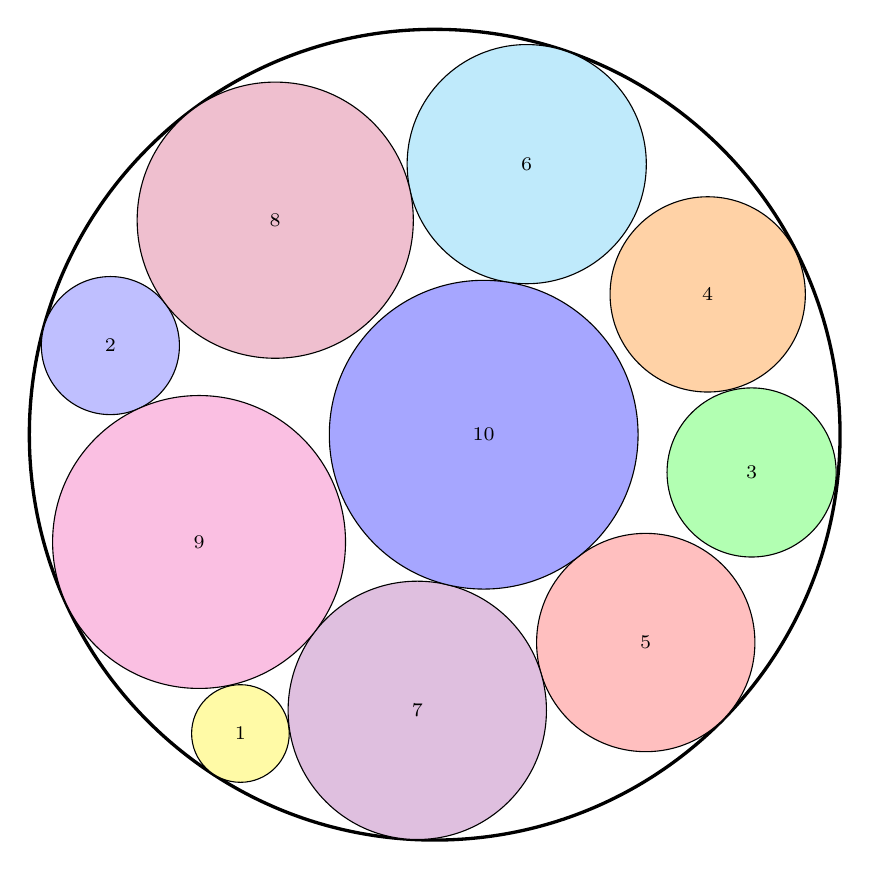
\begin{tikzpicture}[x=0.62cm,y=0.62cm]
  \draw[very thick] (0,0) circle (8.303468122111490);
  \draw[fill=yellow!35,draw=black] (-3.979411598680,-6.120824420924) circle (1.0000);
  \node at (-3.979411598680,-6.120824420924) {\scriptsize 1};
  \draw[fill=blue!25,draw=black] (-6.643004688846,1.825463528216) circle (1.4142);
  \node at (-6.643004688846,1.825463528216) {\scriptsize 2};
  \draw[fill=green!30,draw=black] (6.491367788756,-0.773581798891) circle (1.7321);
  \node at (6.491367788756,-0.773581798891) {\scriptsize 3};
  \draw[fill=orange!35,draw=black] (5.592388025100,2.873904150833) circle (2.0000);
  \node at (5.592388025100,2.873904150833) {\scriptsize 4};
  \draw[fill=red!25,draw=black] (4.323261823214,-4.257082536523) circle (2.2361);
  \node at (4.323261823214,-4.257082536523) {\scriptsize 5};
  \draw[fill=cyan!25,draw=black] (1.885281861457,5.542091227010) circle (2.4495);
  \node at (1.885281861457,5.542091227010) {\scriptsize 6};
  \draw[fill=violet!25,draw=black] (-0.356672093417,-5.646463010751) circle (2.6458);
  \node at (-0.356672093417,-5.646463010751) {\scriptsize 7};
  \draw[fill=purple!25,draw=black] (-3.266260803898,4.394043045277) circle (2.8284);
  \node at (-3.266260803898,4.394043045277) {\scriptsize 8};
  \draw[fill=magenta!25,draw=black] (-4.826665378217,-2.197743262753) circle (3.0000);
  \node at (-4.826665378217,-2.197743262753) {\scriptsize 9};
  \draw[fill=blue!35,draw=black] (1.003716086075,0) circle (3.1623);
  \node at (1.003716086075,0) {\scriptsize 10};
\end{tikzpicture}
\caption{Visualization of the certified upper-bound realization.  The plotted
centers use the rounded coordinates in Table~\ref{tab:upper-coordinates}; the
outer circle has radius $\Rupper$.}
\label{fig:upper-configuration}
\end{figure}

Thus, conditional on the supplementary interval enclosure and Krawczyk
certificate, the configuration gives
\begin{equation}
 \Ropt\le\Rupper.
\end{equation}
Because containment is monotone in the container radius, a configuration
feasible at $R_{\mathrm{root}}$ is also feasible at the larger finite-decimal
radius $\Rupper$.
This is a feasible-witness statement, not an optimality claim.

\section{Conclusion and open problems}

Combining the certified lower bound with the feasible witness gives
\[
 \boxed{7.9\le \Ropt\le
 8.303468122111490.}
\]
The next proof-critical tasks are a global exclusion for every radius below
$\Rupper$, complete treatment of minimal positive stress supports including
degenerate cases, and rigorous extension tests for circles not contained in a
candidate stressed support.  The current result does not assert
$\Ropt=\Rupper$; the displayed upper bound is not claimed to be optimal.

\end{document}
